\documentclass{article}

\usepackage[utf8]{inputenc}
\usepackage[margin=2cm]{geometry}
\usepackage{multicol}
\usepackage{float}
\usepackage{graphicx}
\graphicspath{{images/navigation/}{images/app/}}

\title{Software Design Study Report}
\author{A-Team}

\begin{document}
\maketitle

%\begin{multicols}{2}
\section{Introduction}
\section{Overall system design}
\subsection{Overview}
\subsubsection{Algorithms}
  \begin{itemize}
      \item Bidirectional A* Algorithm
          \begin{itemize}
              \item Heuristics
          \end{itemize}
      \item K means algorithm --- grouping convoys
      \item Learning algorithm --- user preferences, Contextually Aware Routing etc
      % FIND A LEARNING ALGORITHM
      \item Safety Detection algorithms
        \begin{itemize}
            \item Head pose algorithm
            \item Tesla radar system?
            \item Recognising bikes -- trained from training images which are bikes with riders
            % This is if we are detecting bikes using this method of detecting bikes (we mentioned using the 360 degree vision from the cameras for seeing bikes)
        \end{itemize}
      
  \end{itemize}

\subsubsection{Data Structures}
For our navigation algorithm we decided to model the map as a set of nodes and edges where junctions, the start and the destination are nodes and the edges are the roads between these nodes.

    %%%%%%%%%%%%%%%%%%%%%
	%	PLAN
    %%%%%%%%%%%%%%%%%%%%%
  \begin{itemize}
      \item Navigation: Graph --- Representing streets and junctions as edges and nodes
      \item Navigation: Route
	  \item Profile Data
      \item Dashboard layout?
      \item Database --- SQLite for app storage    
  \end{itemize}

\subsubsection{Storage}
  \begin{itemize}
      \item Cloud storage - Oracle Database
          \begin{itemize}
          	  \item Updated from the car and app
              \item User Profiles
              % What is stored here, Car Loc, Settings, Routes (synced with phone), Privileges, seat preferences, driver stats 
              \item Convoy Groups
              % Data on member locations, group messages, routes, route changes etc
              \item Software updates
          \end{itemize}
      \item Car SSD Storage
      \begin{itemize}
      		\item Cached data from the cloud
            \item Cached data from applications such as Spotify
            \item Local music files
            \item Synchronised contacts from phone
            \item Dash cam footage
      \end{itemize}
  \end{itemize}

\subsubsection{Communications}
Within our whole system we have communications between the Mobile App, the Car and our Cloud. 
  \begin{itemize}
      \item Communications between car and phone
      \begin{itemize}     
        	\item NFC pairing for Bluetooth and Wi-Fi
            \item Navigation history shared between app and car to improve destination suggestions
            \item Remote Control
            \item Media Control -- Song requests etc.
	  \end{itemize}
	  \item Communications between car and cloud (Over in-car LTE and external Wi-Fi if available)     	
        \begin{itemize}
          \item Synchronisation with user profiles
          \item System updates
          \item Map updates
          \item Streaming camera feeds
          \item API calls to the cloud
          \item Real time event data, for example someone is breaking into your car, car stats (warning lights)
        \end{itemize}
      \item Communications between phone and cloud      
        \begin{itemize}
        	\item Hashes and timestamps are compared on the server to decide what to synchronise
            \item API calls to the cloud
            \item Car camera feeds can be streamed to the phone on-demand over RTSP
            \item Information regarding convoy setup on phone
            \item Car software updates from cloud (Gives ability to update car with phone)
            \item Real time event data from cloud eg someone breaking into your car, car stats (warning lights)
        \end{itemize}
	  \item Communications between car and external APIs (API links and mappings provided from cloud)
        % Talk about how it connects to the cloud which provides a link to the APIs       
        \begin{itemize}
        	\item Roadworks
            \item Traffic
            \item Weather
            \item Public Transport
            \item Note: All API calls are relative to the country the car is located in.
        \end{itemize}
	\end{itemize}

\subsubsection{Security}
	\begin{itemize}
		\item Database encryption in the cloud
        \item HTTPS for all internet communications
        \item WPA2-PSK with AES for Wi-Fi hotspot login
        \item X.509 certificate for the car
	\end{itemize}

\subsubsection{Interaction Design}
The interaction designs used on our product's interfaces were designed loosely based on designs from industry leading companies but tailored to integrate our ideas and implement some recurrent suggestions found throughout our research, which has seen over 100 responses.

    %%%%%%%%%%%%%%%%%%%%%
	%	PLAN
    %%%%%%%%%%%%%%%%%%%%%
    \begin{itemize}
      \item Centre console
      \item Mobile phone
      \item Rear side door device
      % Justifications of why we have chosen these interfaces
    \end{itemize}
\subsubsection{Aesthetics/Graphical Design}
% User Interfaces of the above devices
An effort was made to follow current styling standards used in industry to give the user a familiar experience, therefore flat designs were used where possible. Also characterising our design are large icons and avoidance of large swathes of text.  
    
    %%%%%%%%%%%%%%%%%%%%%
	%	PLAN
    %%%%%%%%%%%%%%%%%%%%%
    \begin{itemize}
		\item Centre console
        \item Smaller navigation console above centre console
        \item Mobile phone
        \item Rear side door device
        % Justifications of why we have chosen these designs
	\end{itemize}
\section{Feature 1: Navigation}
\subsection{Research}
  \begin{itemize}
    \item Questionnaires
    \item Researching latest technology
  \end{itemize}
\subsection{Brainstorming}
	\begin{itemize}
		\item Collectively worked together to put down all of our ideas into a google doc
		\item No ruling out of ideas
		\item Finally moved everything into a final document. Discussed in a group on each point on whether it should be added or not
        \item Things specific to the nav brainstorm i.e. the ideas to come out of it
	\end{itemize}
\subsection{Tech background}
(Most of this seems like it would be algorithms again, so we plan to expand on the algorithms further than was detailed in section 2.1.1)
  \begin{itemize}
    \item Bidirectional A* search
    \item K-means clustering
  \end{itemize}
  % Include limitations of the above and how we combat them
\subsection{Design choices \& argumentation}
  \begin{itemize}
    \item QOC
    \item Justification for algorithms
    % Would this be better placed in the previous section?
      \begin{itemize}
        \item Routing
        \item Clustering
      \end{itemize}
  \end{itemize}
\subsection{Prototypes \& user testing}
\begin{itemize}
	\item Lo-Fi and Hi-Fi prototypes of Navigation
\end{itemize}
\subsection{Final design}
\subsection{Evaluation \& how it fits into whole system}

\section{Feature 2: App}
\subsection{Research}
Research and brainstorming were conducted in a cyclic manner to ensure that the latest technologies relevant to this sector of the automotive industry were taken into consideration. Extensive research revealed that most leading companies such as Jaguar, BMW and Tesla already offer multi-platform mobile apps that compliment their automobiles. Each of the the above boasts at least one of the features that we intended to integrate in our system such as remote control and seamless route porting from smartphone to car. From brainstorming through to coding the prototype, our focus was directed on how to improve on existing products and also integrate our novel features. 
The research methods we used include a questionnaire, installing and using manufacturers apps on our mobile devices and browsing their websites
	\begin{itemize}
		\item Existing apps that accompany a car
        \item Current technology
		\item How personas might want to interact with an app
        % Link to a persona document in the appendix
	\end{itemize}
\subsection{Brainstorming}
	\begin{itemize}
    	% First 3 points are same as section 3.2
		\item Collectively worked together to put down all of our ideas into a google doc
		\item No ruling out of ideas
		\item Finally moved everything into a final document. Discussed in a group on each point on whether it should be added or not
        \item Things specific to the app brainstorm i.e. the ideas to come out of it
	\end{itemize}
\subsection{Tech background}
	\begin{itemize}
		\item Communication
        \begin{itemize}
        	\item (See section 2.1.4?)
        	\item To and from car
            \begin{itemize}
            	\item Initial connection with the car (Bluetooth/Wifi/RFID)
                \item Communicating remote control instructions
                \item Other instructions (Media control, Controlling hardware)
            \end{itemize}
            \item To and from Cloud
            \begin{itemize}
            	\item Authenticating User profiles
                \item Syncing data
                \item Feeds which are streamed (Camera feeds, )
                \item Information such as Car location
            \end{itemize}
        \end{itemize}
        \item 
	\end{itemize}
    % Repeating what is said in communication (2.1.4) ^^
    
\subsection{Design choices \& argumentation}
  \begin{itemize}
    \item QOC (to be made)
  \end{itemize}
\subsection{Prototypes \& user testing}
  \begin{figure}[H]
    \centering
    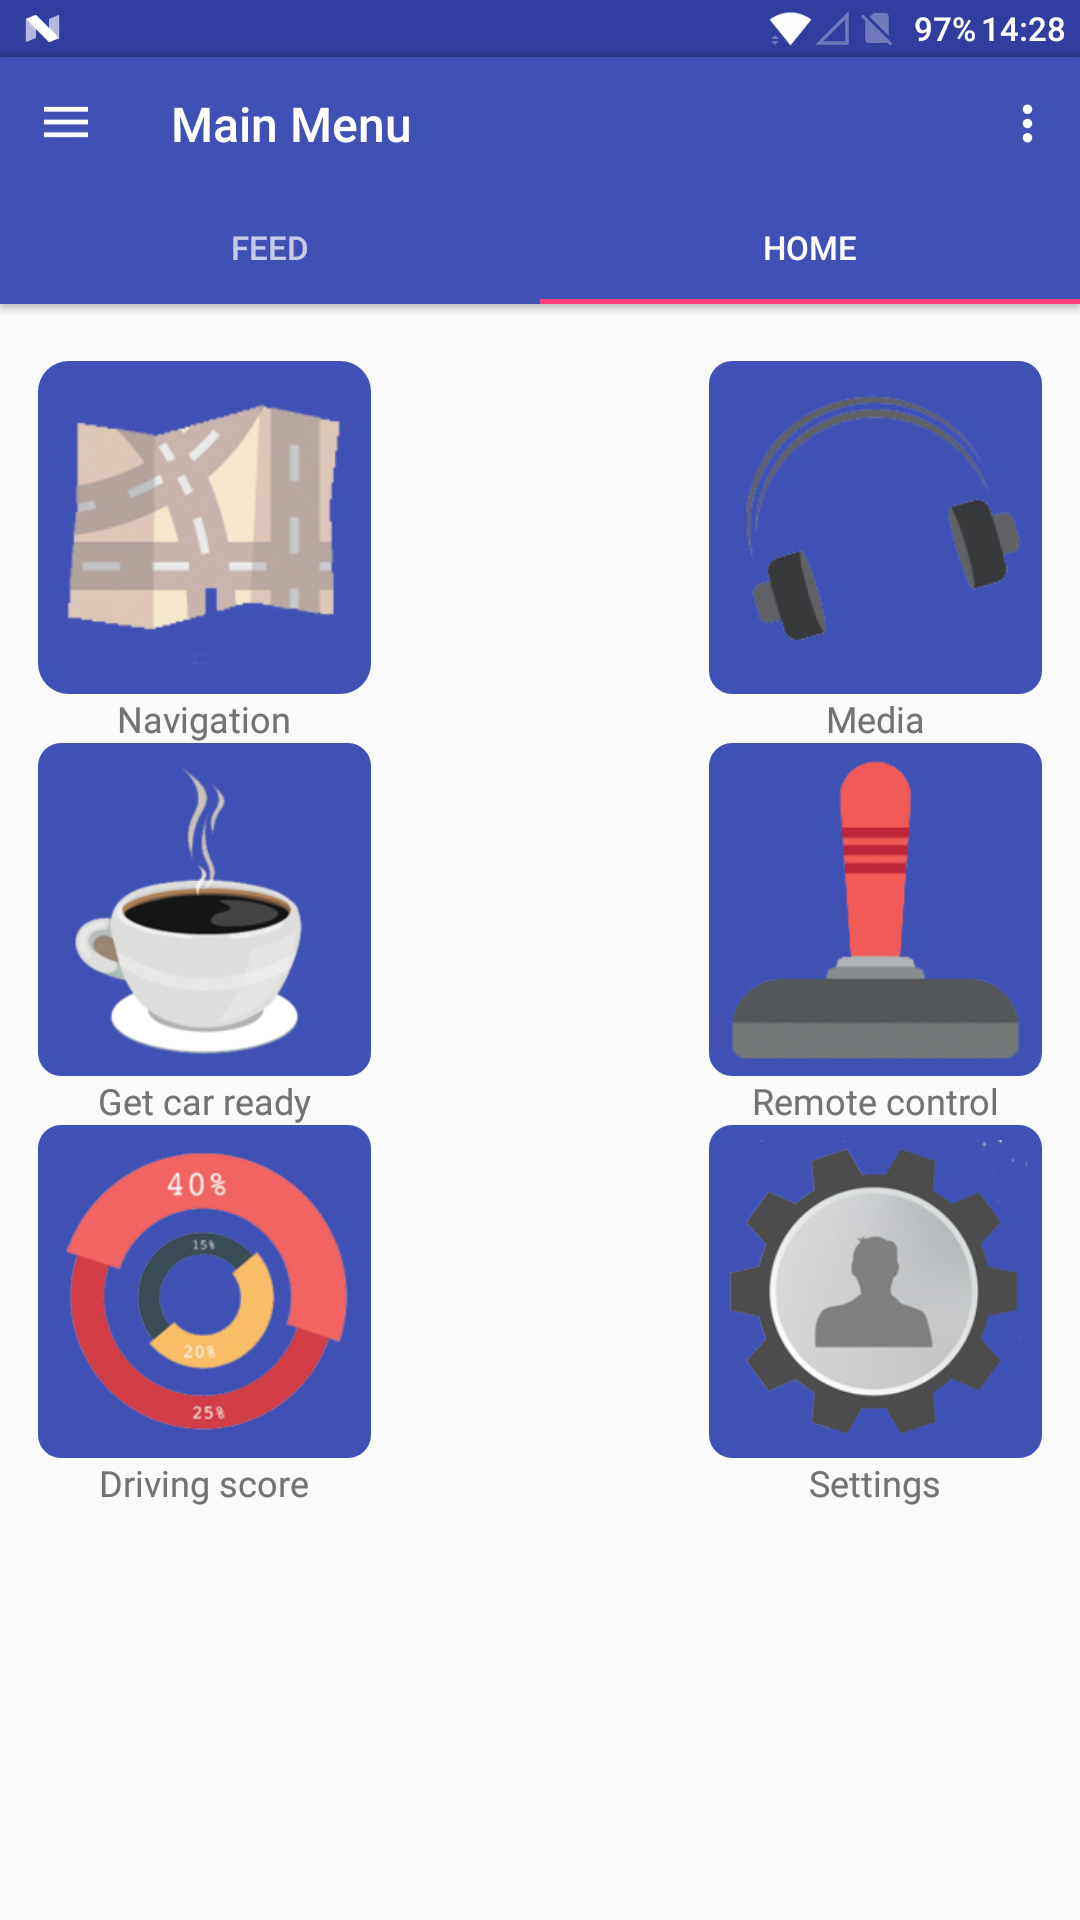
\includegraphics[scale=0.25]{main-menu}
    \caption{Hi-Fi prototype of app main menu.}
    \label{main-menu}
  \end{figure}
\subsection{Final design}
\subsection{Evaluation \& how it fits into whole system}
\section{Other areas}
Annotate slides on changes we would make going forwards
\section{References}
%\end{multicols}
\end{document}
